\documentclass[12pt]{article}

\usepackage{sbc-template}
\usepackage{graphicx,url}
\usepackage[brazil]{babel}
\usepackage[utf8]{inputenc}
\usepackage{listings}

\sloppy

\title{Relatório sobre a Implementação de Comunicação Remota via gRPC com Python}

\author{Julia da Rosa\inst{1}}


\address{Instituto Federal Catarinense -- Campus Rio do Sul -- Unidade Urbana
  (IFC)\\
  \email{julia.rosa.ifc.riodosul@gmail.com}
}

\begin{document} 

\maketitle

\begin{abstract}
  TODO
\end{abstract}
     
\begin{resumo} 
  TODO
\end{resumo}

\section{Introdução}

Neste relatório estaremos explorando o paradigma de comunicação RPC, observando como as entidades se comunicam em um sistema distribuído através de um exemplo didático e funcional em Python utilizando gRPC.

\section{Chamada de Procedimento Remoto (RPC)}

A Chamada de Procedimento Remoto (RPC, do inglês Remote Procedure Call) constitui um mecanismo essencial na computação distribuída, permitindo que procedimentos localizados em máquinas remotas sejam invocados como se estivessem no mesmo espaço de endereçamento do processo cliente.

Esse modelo abstrai os detalhes da comunicação em rede, ocultando processos complexos como a codificação e decodificação de parâmetros, a troca de mensagens entre os nós da rede e a manutenção da semântica de chamadas locais. Dessa forma, o RPC fornece uma camada de transparência que facilita o desenvolvimento de aplicações distribuídas.

A abordagem RPC é especialmente adequada para arquiteturas cliente-servidor, uma vez que os servidores disponibilizam operações por meio de interfaces bem definidas, e os clientes podem invocá-las diretamente, de maneira transparente, como se fossem funções locais.

Do ponto de vista de Sistemas Distribuídos, o gRPC permite a criação de sistemas robustos, desacoplados e eficientes, fundamentais para arquiteturas modernas como microserviços.


\subsection{gRPC}
Para a implementação foi escolhido o gRPC, uma estrutura de RPC de código aberto desenvolvida pela Google que utiliza HTTP/2 para transporte e Protocol Buffers (Protobuf) para serialização de mensagens, oferecendo alta performance e suporte a várias linguagens. Sua comunicação é binária, compacta e rápida, com suporte a multiplexação, streaming, compressão e bidirecionalidade.

Além do gRPC ser mais leve e rápido que REST tradicional,(utilizando JSON + HTTP/1.1), a padronização oferecida pela interface que fortemente tipada e automaticamente gerada via .proto facilita a implementação e entendimento do código.

\section{Descrição da Implementação}
Para tornar a aplicação mais intuitiva, optou-se por adotar um cenário didático inspirado em uma padaria. No lugar da terminologia genérica "produzir" e "consumir", foram definidos dois métodos no serviço gRPC:

Assar(ProdutoRequest): simula a produção de um item de padaria, adicionando-o a um estoque (lista interna).

Vender(VenderRequest): representa a venda de um item ao cliente solicitante, retirando-o do estoque.

Esses métodos fazem parte da interface ProdutoService, definida em um arquivo .proto, conforme o exemplo a seguir:
\begin{lstlisting}
	syntax = "proto3";
	
	package produto;
	
	service ProdutoService {
		rpc Assar(ProdutoRequest) returns (ProdutoResponse);
		rpc Vender(VenderRequest) returns (ProdutoResponse);
	}
	
	message ProdutoRequest {
		string nome = 1;
	}
	
	message VenderRequest {
		string solicitante = 1;
	}
	
	message ProdutoResponse {
		string mensagem = 1;
	}
\end{lstlisting}

O servidor, ou no nosso exemplo $padaria.py$, implementa essa interface utilizando a linguagem Python e a biblioteca gRPC. A classe ProdutoService mantém um atributo estoque, que é manipulado pelos dois métodos principais. A seguir, um trecho do método Assar:

\begin{lstlisting}[language=Python]
	def Assar(self, request, context):
	self.estoque.append(request.nome)
	mensagem = f"Produto '{request.nome}' produzido com sucesso!"
	return produto_pb2.ProdutoResponse(mensagem=mensagem)
	
\end{lstlisting}

E, para o método Vender:
\begin{lstlisting}[language=Python]
	def Vender(self, request, context):
	if self.estoque:
	produto = self.estoque.pop(0)
	mensagem = f"{request.solicitante} comprou o produto '{produto}'."
	else:
	mensagem = "Estoque vazio. Nenhum produto para vender."
	return produto_pb2.ProdutoResponse(mensagem=mensagem)
\end{lstlisting}

Dois clientes foram desenvolvidos:

O cliente "$padeiro$" realiza chamadas ao método Assar para adicionar produtos ao estoque.

O cliente "$consumidor$" realiza chamadas ao método Vender, consumindo os produtos disponíveis.

Para executar esse cenário precisamos também preparar o ambiente com a execução do comando ``$python -m grpc_tools.protoc -I=protos --python_out=. --grpc_python_out=. produto.proto$'' no projeto de tal forma que $grpc_python_out$ seja o caminho relativo para o arquivo $produto.proto$ a partir do diretório onde o comando foi executado para que os arquivos $produto_pb2.py$ e $produto_pb2_grpc.py$ sejam criados automaticamente onde o comando foi executado. Esses arquivos devem estar no mesmo diretório onde o servidor, $padaria.py$, está ou em um local visível via import. Para que então o servidor possa ser executado.


\begin{figure}
	\centering
	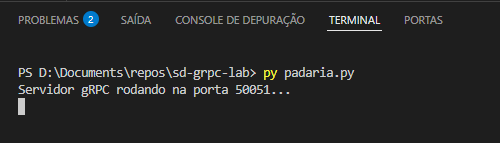
\includegraphics[width=0.6\textwidth]{py padaria.py.png}
	\caption{Executando $py padaria.py$ no terminal.}
	\label{fig:uml}
\end{figure}


\begin{figure}
	\centering
	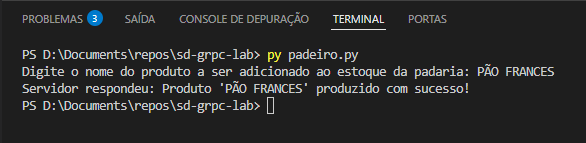
\includegraphics[width=0.6\textwidth]{py padeiro.py.png}
	\caption{Executando $py padeiro.py$ no terminal.}
	\label{fig:uml}
\end{figure}

\begin{figure}
	\centering
	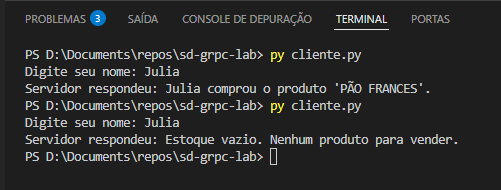
\includegraphics[width=0.6\textwidth]{py cliente.py - sem estoque.png}
	\caption{Executando $py cliente.py - sem estoque.py$ no terminal.}
	\label{fig:uml}
\end{figure}


\section{Conclusão}

TODO

\bibliographystyle{sbc}
\bibliography{referencias}
COULOURIS, George et al. Sistemas distribuídos: conceitos e projeto. 5. ed. Porto Alegre: Bookman, 2013. ISBN 978-85-8260-054-2. 

\end{document}
%\section{General Information}
%
%All full papers and posters (short papers) submitted to some SBC conference,
%including any supporting documents, should be written in English or in
%Portuguese. The format paper should be A4 with single column, 3.5 cm for upper
%margin, 2.5 cm for bottom margin and 3.0 cm for lateral margins, without
%headers or footers. The main font must be Times, 12 point nominal size, with 6
%points of space before each paragraph. Page numbers must be suppressed.
%
%Full papers must respect the page limits defined by the conference.
%Conferences that publish just abstracts ask for \textbf{one}-page texts.
%
%\section{First Page} \label{sec:firstpage}
%
%The first page must display the paper title, the name and address of the
%authors, the abstract in English and ``resumo'' in Portuguese (``resumos'' are
%required only for papers written in Portuguese). The title must be centered
%over the whole page, in 16 point boldface font and with 12 points of space
%before itself. Author names must be centered in 12 point font, bold, all of
%them disposed in the same line, separated by commas and with 12 points of
%space after the title. Addresses must be centered in 12 point font, also with
%12 points of space after the authors' names. E-mail addresses should be
%written using font Courier New, 10 point nominal size, with 6 points of space
%before and 6 points of space after.
%
%The abstract and ``resumo'' (if is the case) must be in 12 point Times font,
%indented 0.8cm on both sides. The word \textbf{Abstract} and \textbf{Resumo},
%should be written in boldface and must precede the text.
%
%\section{CD-ROMs and Printed Proceedings}
%
%In some conferences, the papers are published on CD-ROM while only the
%abstract is published in the printed Proceedings. In this case, authors are
%invited to prepare two final versions of the paper. One, complete, to be
%published on the CD and the other, containing only the first page, with
%abstract and ``resumo'' (for papers in Portuguese).
%
%\section{Sections and Paragraphs}
%
%Section titles must be in boldface, 13pt, flush left. There should be an extra
%12 pt of space before each title. Section numbering is optional. The first
%paragraph of each section should not be indented, while the first lines of
%subsequent paragraphs should be indented by 1.27 cm.
%
%\subsection{Subsections}
%
%The subsection titles must be in boldface, 12pt, flush left.
%
%\section{Figures and Captions}\label{sec:figs}
%
%
%Figure and table captions should be centered if less than one line
%(Figure~\ref{fig:exampleFig1}), otherwise justified and indented by 0.8cm on
%both margins, as shown in Figure~\ref{fig:exampleFig2}. The caption font must
%be Helvetica, 10 point, boldface, with 6 points of space before and after each
%caption.
%
%\begin{figure}[ht]
%\centering
%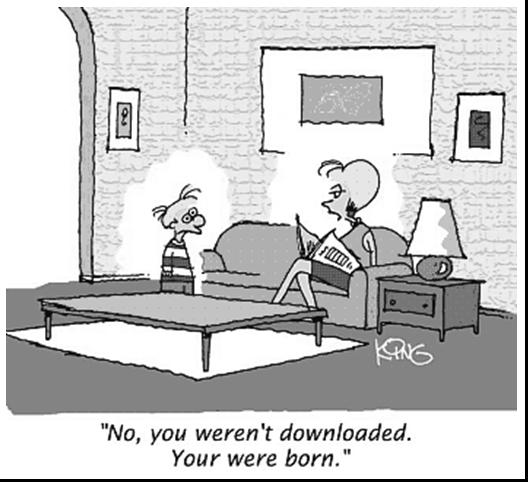
\includegraphics[width=.5\textwidth]{fig1.jpg}
%\caption{A typical figure}
%\label{fig:exampleFig1}
%\end{figure}
%
%\begin{figure}[ht]
%\centering
%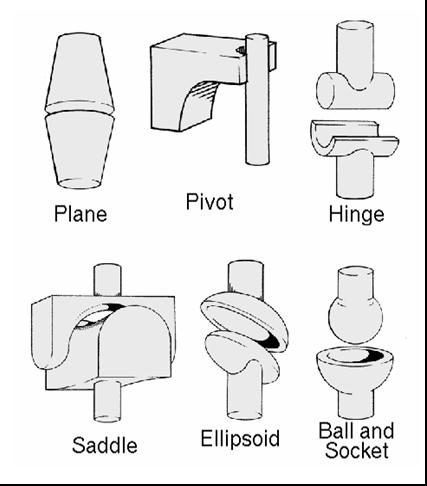
\includegraphics[width=.3\textwidth]{fig2.jpg}
%\caption{This figure is an example of a figure caption taking more than one
%  line and justified considering margins mentioned in Section~\ref{sec:figs}.}
%\label{fig:exampleFig2}
%\end{figure}
%
%In tables, try to avoid the use of colored or shaded backgrounds, and avoid
%thick, doubled, or unnecessary framing lines. When reporting empirical data,
%do not use more decimal digits than warranted by their precision and
%reproducibility. Table caption must be placed before the table (see Table 1)
%and the font used must also be Helvetica, 10 point, boldface, with 6 points of
%space before and after each caption.
%
%\begin{table}[ht]
%\centering
%\caption{Variables to be considered on the evaluation of interaction
%  techniques}
%\label{tab:exTable1}
%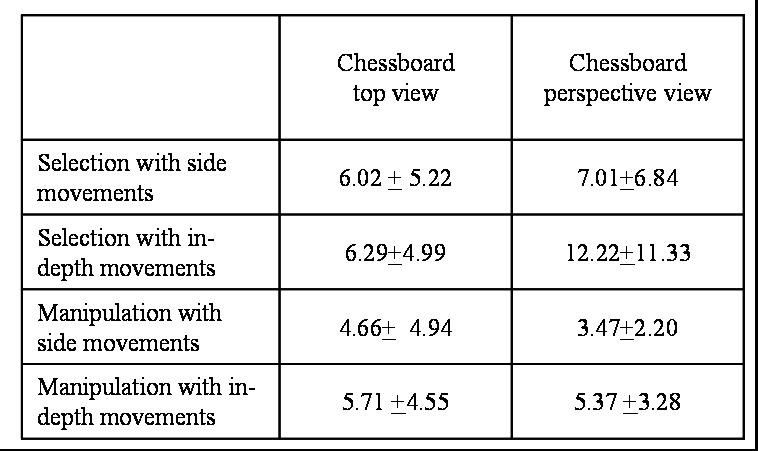
\includegraphics[width=.7\textwidth]{table.jpg}
%\end{table}
%
%\section{Images}
%
%All images and illustrations should be in black-and-white, or gray tones,
%excepting for the papers that will be electronically available (on CD-ROMs,
%internet, etc.). The image resolution on paper should be about 600 dpi for
%black-and-white images, and 150-300 dpi for grayscale images.  Do not include
%images with excessive resolution, as they may take hours to print, without any
%visible difference in the result. 
%
%\section{References}
%
%Bibliographic references must be unambiguous and uniform.  We recommend giving
%the author names references in brackets, e.g. \cite{knuth:84},
%\cite{boulic:91}, and \cite{smith:99}.
%
%The references must be listed using 12 point font size, with 6 points of space
%before each reference. The first line of each reference should not be
%indented, while the subsequent should be indented by 0.5 cm.
%
%\bibliographystyle{sbc}
%\bibliography{sbc-template}
%
%\end{document}
